\documentclass[10pt,landscape]{article}
\usepackage[landscape]{geometry}
\usepackage{multicol}

\usepackage{mathtools}
\usepackage{amsmath}
\usepackage{amsfonts}
\usepackage{xfrac}
\usepackage{graphicx}

% Make the margins tight
\geometry{top=1cm, right=1cm, bottom=1cm, left=1cm}

% remove headers and footers
\pagestyle{empty}

% Make paragraph splits smaller
\setlength{\parindent}{0pt}
\setlength{\parskip}{0.5ex}

% Make the section headings smaller, inspired by the class Latex2e
% quick reference sheet.
\makeatletter
\renewcommand{\section}{\@startsection{section}{1}{0pt}%
                        {-1.3ex}{0.7ex}{\normalfont\large\bfseries}}
\renewcommand{\subsection}{\@startsection{subsection}{2}{0pt}%
                           {-1.3ex}{0.7ex}{\normalfont\normalsize\bfseries}}
\renewcommand{\subsubsection}{\@startsection{subsubsection}{3}{0pt}%
                              {-1.3ex}{0.7ex}{\normalfont\small\bfseries}}
\makeatother

% Tighten-Up lists
\let\oldenumerate\enumerate
\renewcommand{\enumerate}{%
    \oldenumerate%
    \setlength{\itemsep}{0pt}%
}

\let\olditemize\itemize
\renewcommand{\itemize}{%
    \olditemize%
    \setlength{\itemsep}{0pt}%
}

\let\olddescription\description
\renewcommand{\description}{%
    \olddescription%
    \setlength{\itemsep}{0pt}%
}

% Remove section numbers
\setcounter{secnumdepth}{0}

% Utility commands
\newcommand{\spto}{\;\to\;}
\newcommand{\spbar}{\;|\;}
\newcommand{\spbackslash}{\;\backslash\;}
\newcommand{\impl}{\Rightarrow}

% temp length variable
\newlength{\templength}

\begin{document}
\begin{multicols*}{3}

\begin{center}
    \Large CS3100 Final Note Sheet
\end{center}
\vspace{-0.5cm}

\section{Notation}
\begin{tabular}{rp{0.79\linewidth}}
$L^R$ & The reversal of language $L$. \\
$L^*$ & The Kleene-Star of $L$. \\
$AB$ & The concatenation of language $A$ and $B$. \\
$h(L)$ & A homomorphism (a function that maps every input to 
         a unique output) of $L$. \\
$A \spbackslash B$ & Set difference of $A$ and $B$. 
                     $A - B$ is the same thing. \\
\end{tabular}
$f : x_1, x_2, \ldots, x_n \to y_1, y_2, \ldots, y_n$ denotes
a function $f$ that when given $x_1, \ldots, x_n$ as inputs
yields $y_1, \ldots, y_n$ as outputs.

\section{Chomsky Hierarchy}
\begin{center}
    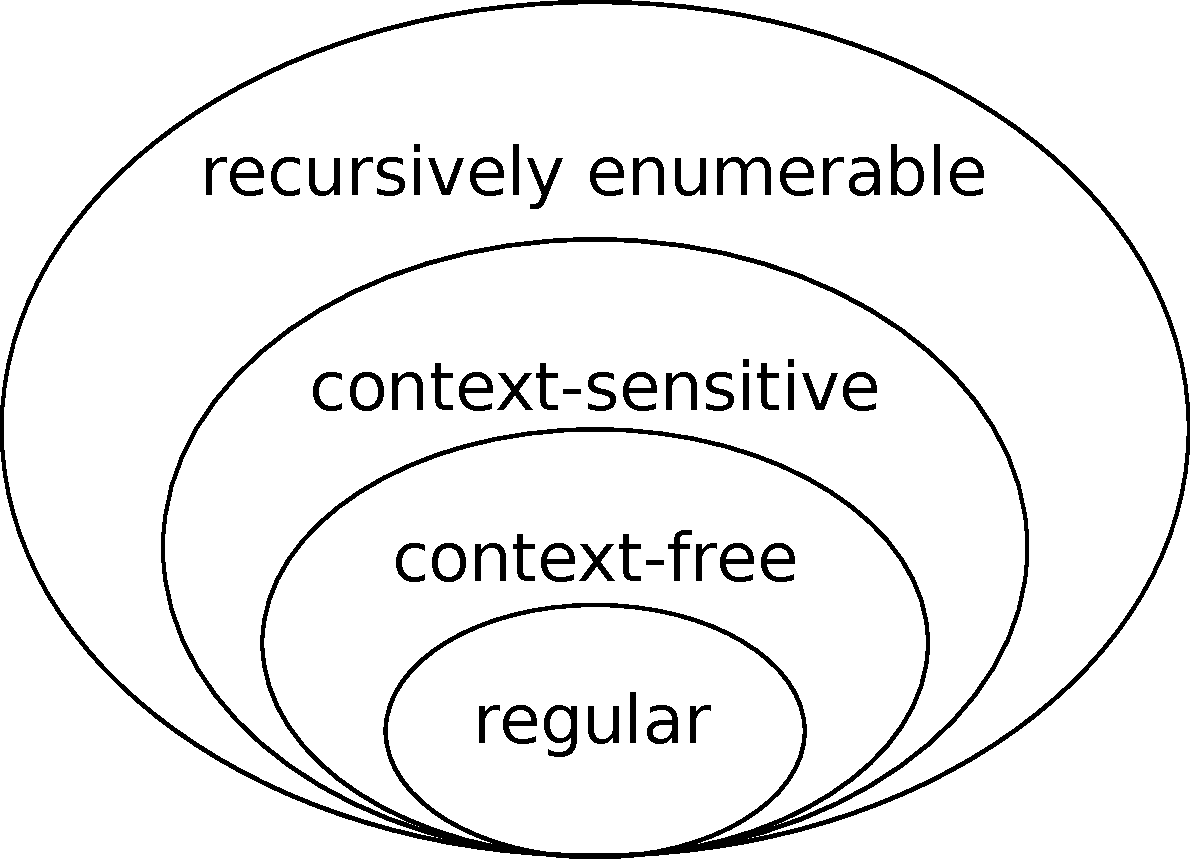
\includegraphics[width=0.6\linewidth]{images/chomsky-hierarchy}
\end{center}

% Regular Languages
% - DFA formalism
% - Talk about NFA/DFA conversion
% - NFA/DFA closures
%   e.g. answer 'how do I reverse an NFA
% - Pumping lemma shortcuts
% -! DFA minimization
% - DFA to RE-conversion
\section{Regular Languages}

A regular language is any language that can be recognized with a DFA.
Formally a DFA is a tuple $(Q,\Sigma,\delta,q_0,F)$. Where:

\begin{tabular}{rp{0.79\linewidth}}
$Q$             & A finite, non-empty set of states. \\
$\Sigma$        & A finite, non-empty alphabet. \\
$\delta$        & A function ($\delta : Q \times \Sigma \to Q$) that maps
                  a state, and an input in $\Sigma$ to a new state. \\
$q_0$           & A state in $Q$ that DFA starts execution from. \\
$F \subseteq Q$ & A finite, possibly empty, set of accepting states.
\end{tabular}

\subsection{Closures}
Where $R$ is a regular language, $L$ is `not regular', and $?$ is Unknown.

% Figure out the width of the third coulumn
\settowidth{\templength}{$R \cap R \spto R$}
\addtolength{\templength}{1cm}
\begin{tabular}{lp{\templength}l}
\textbf{Closed:}       &                    & \textbf{Unclosed:} \\
$\overline{R} \spto R$ & $h(R) \spto R$     & $R \cap L \spto ?$ \\
$R^* \spto R$          & $R \cup R \spto R$ & $R \cup L \spto ?$\\
$R^R \spto R$          & $R \cap R \spto R$ & $L \cup L \spto ?$\\
$RR \spto R$           & $R \spbackslash R \spto R$ & \\
\end{tabular}

\subsection{Pumping Lemma}
\begin{align*}
\exists N \in \mathbb{N}: & \\
         \forall w \in L: &\; |w| \geq N \impl \\
\exists xyz \in \Sigma^*: & \quad w = xyz \\
                          & \land |xy| \leq N \\
                          & \land y \neq \varepsilon \\
                          & \land \forall i \geq 0: xy^iz \in L
\end{align*}

% Context-Free languages:
% - CFL formalism
% - RL and LL to NFA/DFA conversion
%   - RL conversion via reversal closures
% - Shortcuts for solving pumping lemmas
% - Chompsky Normal form
% - CFG -> PDA conversion 
\section{Context Free Languages}

\subsection{Closures}
Where $C$ is a context-free language, $R$ is a regular language, and $?$ is
an Unknown language.

\settowidth{\templength}{$C \cup C \spto C$}
\addtolength{\templength}{1cm}
\begin{tabular}{lp{\templength}l}
\textbf{Closed:} & & \textbf{Unclosed:} \\
$C^R \spto C$ & $C \cup C \spto C$ & $\overline{C} \spto ?$\\
$C^* \spto C$ & $C \cap R \spto C$ & $C \cap C \spto ?$\\
$CC \spto C$  & $C \cup R \spto R$ & $C \spbackslash C \spto ?$\\
$h(C) \spto C$ & & \\
\end{tabular}

\subsection{Pumping Lemma}
\begin{align*}
  \exists N \in \mathbb{N}: & \\
          \forall w \in L : & |w| \geq N \impl \\
\exists uvxyz \in \Sigma^*: & \quad w = uvxyz \\
                            & \land |vy| > 0 \\
                            & \land |vxy| \leq N \\
                            & \land \forall i \geq 0: uv^ixy^iz \in L
\end{align*}

\subsection{Ambiguous Context Free Languages}
These are languages that have two separate parse-trees. To prove
that a language is ambiguous, show that it actually has two separate
parse-trees.

Example ambiguous grammar:
\[
    E \spto E + E \spbar E * E \spbar \texttt{NUMBER}
\]
% TODO: Needs graph example

\subsection{Consistency and Completeness}
\begin{description}
    \item[{\small Consistency:}] All strings generated by a grammar are 
    in the language.
    \item[{\small Completeness:}] The grammar generates all strings 
    in the language.
\end{description}

You cannot know that a grammar defines a language until you show both.
For example, if we want to define the language $\{a^nb^n | n \in \mathbb{N}\}$,
the grammar:
\[
    S \spto aabb
\]
Is \textit{consistent} because it only generates strings in the language,
but not complete because it doesn't generate all strings in the language.
Likewise, the grammar:
\[
    S \spto aS \spbar bS \spbar \varepsilon 
    \;\;\quad (\textit{grammar for }\{a, b\}^*)
\]
Is complete, it generates all possible strings in the language, but not
consistent because it generates many strings that are, in-fact, outside of
the language.

% Cardinality
% (mostly done) Schroder-Bernstein theorem
% - Cardinality using a paring function.
\section{Cardinality}
\subsection{Schr\"{o}der-Bernstein Theorem}
The Schr\"{o}der-Bernstein theorem states that, for any two sets $A$ and $B$
if there exists an \textit{injective} function from $A \to B$, and
there exits an injective function from $B \to A$, then $|A| = |B|$.
Note that the injective function doesn't require every item of $A$ to map
to every item of $B$, only that every item of $A$ maps to \textit{an} item
of $B$ (and vice versa).

% Turing Machines
% - TM formalism
% - How to make a Turing machine 
% - DTM / NDTMs
% - Turing Machine terminology (acceptance, halting, rejection, deciders)
\section{Turing Machines}
\subsection{Terminology and Notation}
\begin{tabular}{rp{0.71\linewidth}}
$\langle M \rangle$ & String representation of Turing machine $M$. \\
halting & When a machine stops execution. \\
acceptance & When a machine halts in a final state. \\
rejection & When a machine halts and is not in a final state. \\
decider & A decider is a Turing machine that defines a language
          of Turing machines that conform to a yes or no question. \\
\end{tabular}

\section{Decidability}
\subsection{Halting Problem}
The halting problem states building a Turing machine $P$ that can detect
whether any other Turing machine will halt is impossible. The proof is as
follows:

Assume that we have a Turing machine $P$, that when given a Turing machine
$M$ and string $w$ as input ($\langle M, w \rangle$), $P$ will (in a finite
computation time) accept in the case that $M$ halts on input 
$w$, or reject in the case that $M$ loops on input $w$. We can then
define a new Turing machine $Q$ that takes a single Turing machine $M$ 
as input. $Q$ will then ask $P$ whether machine $M$ halts when given
itself as input (does $P(\langle M, M \rangle)$ halt?). If $P$ 
accepts (says that $M$ halts) the $Q$ will loop. If $P$ rejects 
(says $M$ will loop) then $Q$ halts. Now, we can supply $Q$ as input
to machine $Q$. $Q$ will then run $P(\langle Q, Q \rangle)$. If $P$
accepts, then $Q$ will begin to loop, but $P$ said that $Q$ would
halt. This is a contraction, a general $P$ decider for the halting problem
cannot exist.

\subsection{Mapping Reduction}
A mapping reduction between $A \subseteq \Sigma^*$ and 
$B \subseteq \Sigma^*$ is a function $f : \Sigma^* \to \Sigma^*$ if
$\forall x \in \Sigma^*, x \in A \Leftrightarrow f(x) \in B$. More plainly,
a function $f$ such that I can pick any $x$ in $A$, and $f(x)$ will also
be in $B$. The ``mapping reduction from $A$ to $B$'' is typically denoted
as $A \leq_m B$. A mapping reduction in polynomial time is denoted
$A \leq_p B$.

The general steps for a mapping reduction $A \leq_m B$ are as follows:
\begin{enumerate}
    \item $A$ is designated the ``known undecidable'' language.
    \item $B$ is designated the ``unknown'' language.
    \item Create a function $f$ that maps all elements of $A$ into $B$.
\end{enumerate}

To form $f$ you usually assume the decider for $B$ ($D_B$), then you construct
a machine $M$ that uses to decider $D_B$ to become a decider for $A$ ($D_A$).
For example, we can map $A_{TM}$ onto $Halt_{TM}$ using the following method:

Assume that a decider $R$ for $A_{TM}$ exists. We will now construct
a decider $S$ for $Halt_{TM}$ from $R$. $S$ has two inputs a machine $M$ and
an input string $w$. First, $S$ will run decider $R$ on $\langle M, w$,
if $R$ accepts, then $S$ accepts. If $R$ rejects, then $S$ accepts. We
now have a decider for $Halt_{TM}$ which is undecidable, a decider for
$A_{TM}$ cannot exist.

\subsection{Rice's Theorem}
``Every non-trivial partitioning of the space of Turing machine 
codes based on the languages recognized by these Turing machines 
is undecidable.''

More formally, given a property $\mathcal{P}$, where $\mathcal{P}$ is
non-trivial (not $\emptyset$ or $\Sigma^*$) the language below is
undecidable.
\[
    {\langle M \rangle \spbar M \text{ is a Turing machine and } 
        \mathcal{P}(Lang(M))}
\]

% NP-Completeness
% - Definitions of P, NP, NP-complete, and NP-hard.
% - Talk about Turing verifiers (For showing L is in NP)
% - Talk about how to prove a language is NP-complete
\section{NP-Completeness}
\subsection{Problem Classes}
\begin{description}
    \item[{\small P:}] The set of problems that can be solved
    in polynomial time. Contained in NP.
    \item[{\small NP:}] The set of problems that can be solved
    in non-deterministic polynomial time.
    \item[{\small NP-hard:}] The set of problems that can be
    polynomial time reduced to every other problem in NP.
    \item[{\small NP-complete:}] The set of problems that are
    in both NP, and NP-hard.
\end{description}
\subsection{Proving NP-Completeness}
There are two steps to proving that a languages is in NP-complete.
First you have to show that it is NP, and then you have to show that
it is in NP-hard.

\subsubsection{Verifiers}
One way to show that a problem is in NP is by using a verifier. A verifier
is a Turing machine $V_L$ such that for all $w \in \Sigma^*$, their exists
some $c$ such that $w \in L$ when $V_L(w, c)$ accepts. Intuitively this can
be understood as ``There is a machine that can check the answers to problems
quickly''.

\subsection{NP-hard Reduction}

\end{multicols*}
\end{document}
